%  Discussion.tex
% !TeX spellcheck = en_GB
% !TeX root = ReportMain.tex

\section{Discussion} \label{s:Discussion}
Comparison and discussion (Suggestions on improvement).
%BH
\subsection{Success Criteria}
What are the values the design must pass?

\subsection{No Foils}
\begin{figure}[!h]
  \centering
    \includegraphics[width = 0.8\textwidth]{../Simulations/DataSets/No_Foil_Fail.eps} 
\caption{The No Foils Model Fails PD Criteria}
\label{Figure:NoFoilsFail}
\end{figure}

\subsection{No Grading}

\subsection{Comparison of Axial and Radial Grading Solutions}
The design of both types of capacitive grading method were discussed in the previous sections. The difference in performance of the types in general is the radial grading will improve the intensity of the radial electric field and the axial grading will improve the intensity of the axial electric field. By improvement of intensity of electric field, this means the electric field according to the type of grading method is evenly distributed in a particular direction. Choosing the right design for different application is essential as this will reduce the chances of various types of electrical breakdown and hence the bushing design would be more durable.

There are two components of electric field cause different problems. The radial electric field is mainly responsible to the breakdown of insulating material, for example, electrical breakdown between foils. On the other hand, the axial electric field is mainly responsible to the surface discharges along the boundary of the insulation, for example, corona discharge to the surrounding.

\subsubsection{Radial Electric Field}
The maximum intensity of the radial electric field for the radial design is expected to be lower than the maximum of the axial design. This means the radial grading design would perform better to suppress the intensity of radial electric field. The radial electric field across the radial direction of both axial and radial grading designs are shown in figure \ref{figure:rfield}.

\begin{figure}[!h]
\centering
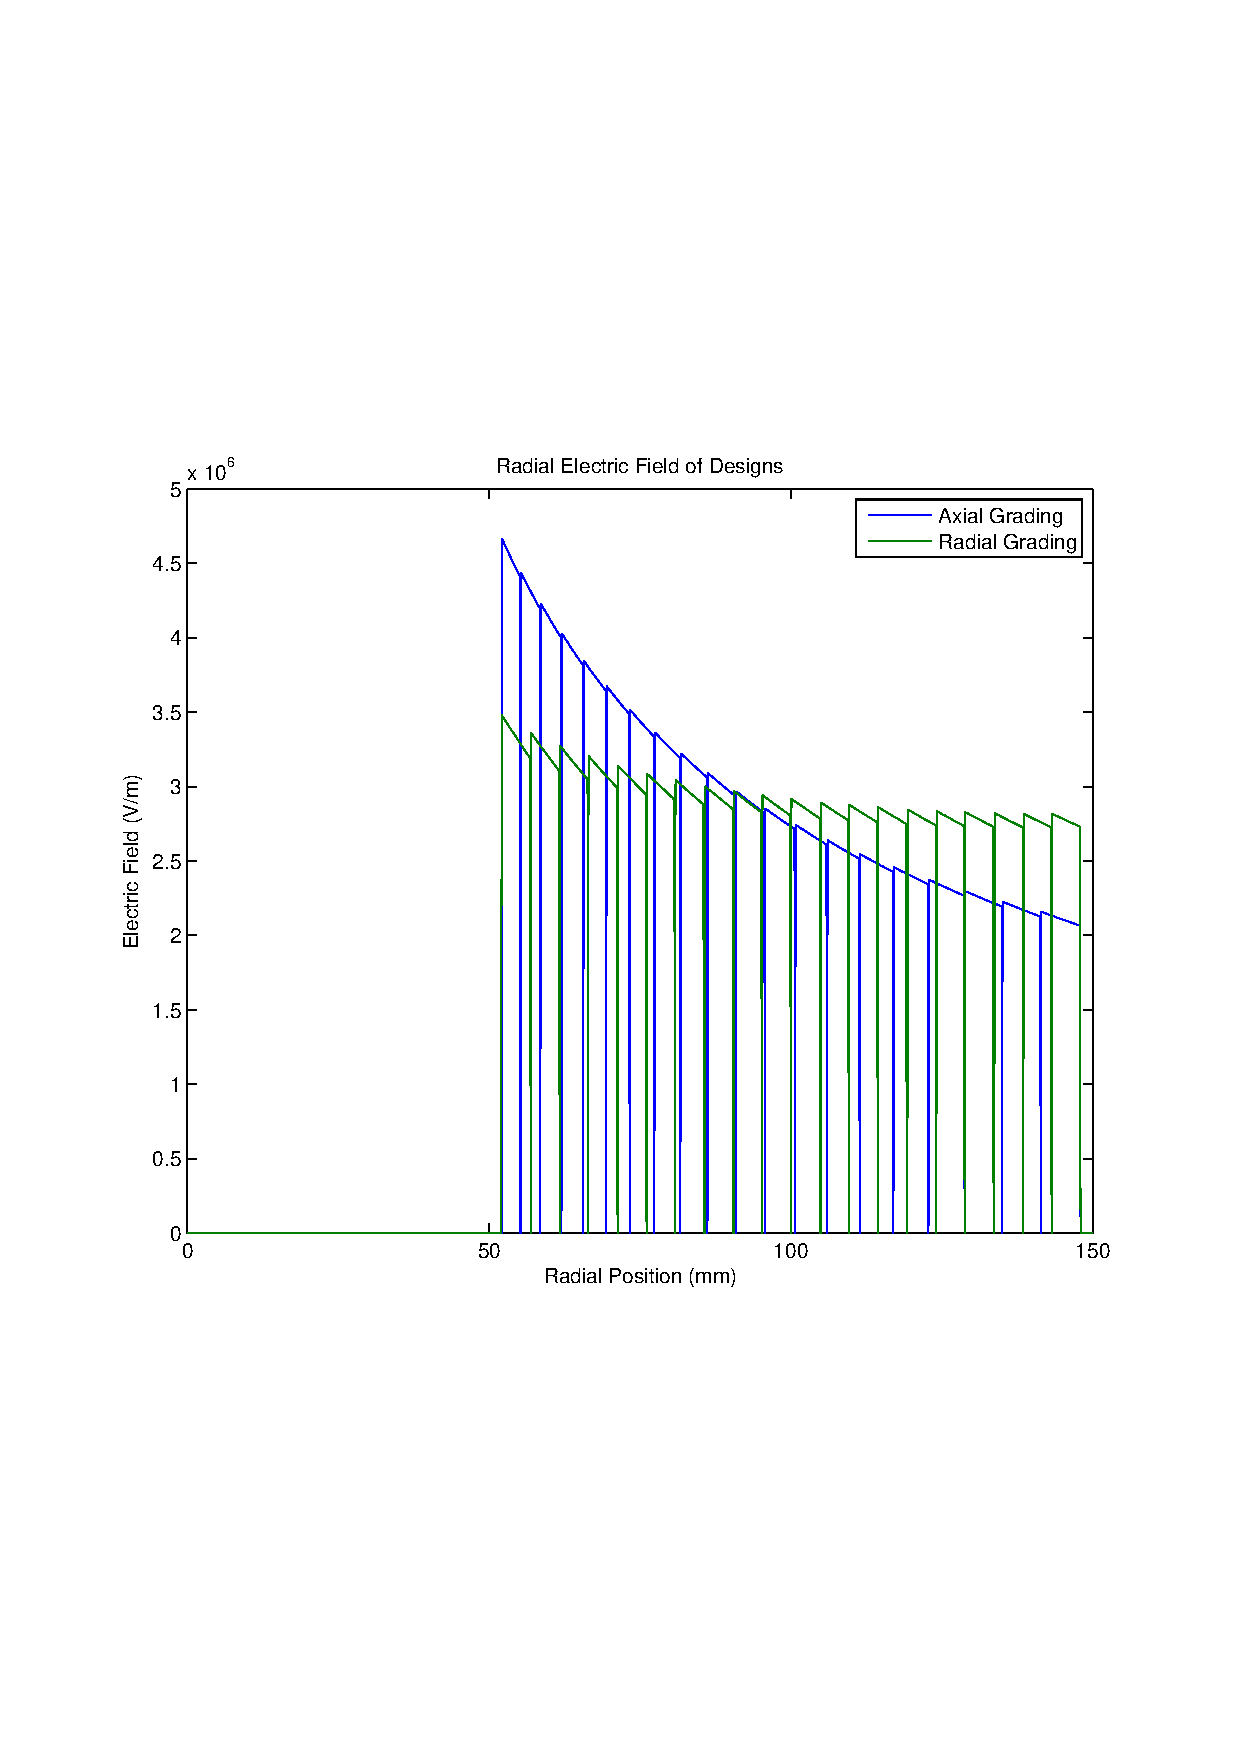
\includegraphics[width = \textwidth]{R-field.jpg}
\caption{Radial electric field across the mid-point of the two designs of bushing.}
\label{figure:rfield}
\end{figure}

The result clearly shows the peak value of electric field for the axial design ($\approx 4.5 \times 10^3 kVm^{-1}$) is greater than the peak value of electric field for the radial design ($\approx 3.5 \times 10^3 kVm^{-1}$). Also, from the figure \ref{figure:rfield}, the radial electric field of the radial grading design is more evenly distributed. This is the effect of grading, hence similar effect should be seen in the axial electric for axial grading design. The electric field distribution across any perpendicular cut lines to the foils would result in almost identical results, because the foils behave similar to capacitors in series. Electric field being constant across a capacitor and this is true across any two neighbouring foils.

\subsubsection{Axial Electric Field}
The axial component of electric field is responsible for the surface discharges along the surface of the bushing design. Axial component of the field contributes to these surfaces, because the axial electric field at the edges of the foil are the most intense. Figure \ref{figure:afield} shows the magnitude of electric field at each foil edge. 

\begin{figure}[!h]
\centering
\includegraphics[width = \textwidth]{A-field.jpg}
\caption{Electric field at the edge of each foil.}
\label{figure:afield}
\end{figure}
%this graph is a mess, I took very long time to convince myself to put this on here. This is the best I can do at the moment

The result clearly shows the radial design has a lower peak value of electric field at these edges of foil. However, this is not an expected result, because axial grading in theory shapes the surface of the insulation better to avoid intensifying of electric field at these edges. Also, a clearer maximum peak of electric field at should be seen at the outermost foil of the radial graded design due to the sharp turn in the shape of the bushing design. Although the result shows a maximum peak at the last outermost foil, it is not significant and it is below the maximum value of electric field for the axial graded design.

\subsubsection{Surface Flashover}
Surface flashover is the partial discharge along the surface of the insulation, this is cause by a intense electric field. The parameter which takes into account of surface flashover is the creepage distance. The typical value for creepage distance is 35mm/kV %need a reference for this prob%
and for more polluted environment, a higher value of creepage distance might be considered.

In bushing designs, 

\subsection{Choice of Design Method}

\section{Conclusions}
Conclusions.